\documentclass[11pt,a4paper]{article}

\usepackage[margin=2.1cm]{geometry}
\usepackage[T1]{fontenc}
\usepackage{lmodern}
\usepackage{microtype}
\usepackage{graphicx}
\usepackage{booktabs}
\usepackage{tabularx}
\usepackage{multirow}
\usepackage{array}
\usepackage{xcolor}
\usepackage{listings}
\usepackage{enumitem}
\usepackage{caption}
\usepackage{float}
\usepackage{tikz}
\usetikzlibrary{positioning,arrows.meta,fit,backgrounds}
\usepackage{pgfplots}
\pgfplotsset{compat=1.18}
\usepgfplotslibrary{groupplots}
\usepackage[hidelinks]{hyperref}

\setlist{itemsep=2pt, topsep=4pt}
\captionsetup{font=small, labelfont=bf}
\renewcommand{\arraystretch}{1.15}
\newcolumntype{L}{>{\raggedright\arraybackslash}X}

\definecolor{codebg}{RGB}{248,248,250}
\definecolor{cA}{RGB}{31,119,180}
\definecolor{cB}{RGB}{255,127,14}
\definecolor{cC}{RGB}{44,160,44}
\definecolor{cD}{RGB}{148,103,189}
\lstset{
  basicstyle=\ttfamily\footnotesize, backgroundcolor=\color{codebg},
  frame=single, rulecolor=\color{gray!40}, breaklines=true, showstringspaces=false,
  columns=fullflexible, xleftmargin=0.5em
}

\newcommand{\repo}{https://github.com/Rahul5977/CSD-Course/tree/main/Lab-Task/10.FiOTools}

\title{\textbf{Lab 10: Simulating PostgreSQL Storage Workloads with FIO}}
\author{Rahul Raj \quad (12341680)\\\small CS559 System Design}
\date{\today}

\begin{document}
\maketitle

\begin{center}
\begin{tabularx}{\linewidth}{@{}lL@{}}
\toprule
Database studied & PostgreSQL 16 (current major version at the time of writing; 8 KiB pages, WAL, buffered I/O) \\
Use case & OLTP order/payment service with a nightly reporting job \\
Tool & fio 3.36 (Ubuntu 24.04 package), \texttt{libaio}, \texttt{direct=1} \\
Machine & MacBook, Apple M4, 16 GiB RAM, internal Apple SSD; Docker Desktop 29.1.3 (Linux VM: kernel 6.12.54-linuxkit, 10 vCPU, 7.7 GiB) \\
Target & 1 GiB file on ext4 in a dedicated Docker volume (\texttt{/fio-lab}, virtio disk \texttt{vda}) \\
Code \& raw data & \href{\repo}{\texttt{github.com/Rahul5977/CSD-Course}}, folder \texttt{Lab-Task/10.FiOTools} \\
\bottomrule
\end{tabularx}
\end{center}

% ---------------------------------------------------------------------------
\section{Chosen database and its expected workload}

\textbf{Database: PostgreSQL 16.} I picked it because its storage behaviour is well documented and maps
cleanly onto the four required FIO patterns. Each part of it does a distinct kind of I/O:
\begin{itemize}
  \item tables (heap) and B-tree indexes are stored as files of fixed \textbf{8 KiB pages};
  \item every change is first appended to the \textbf{write-ahead log (WAL)} and flushed at commit;
  \item dirty pages are written back to the data files later, out of order, by the
        \emph{checkpointer} and \emph{background writer};
  \item PostgreSQL 16 uses \textbf{buffered I/O}: a page that misses \texttt{shared\_buffers} is
        requested from the kernel and may still be served from the OS page cache.
\end{itemize}
That gives one random read path, one random write path and one sequential append path to model.

\textbf{Intended use case.} An OLTP order/payment service (``look up customer, read product rows,
insert an order, update stock'') plus a nightly reporting query that scans the orders table.
The database is assumed to be larger than RAM, so a share of page reads reach storage.

\noindent{\small
\begin{tabularx}{\linewidth}{@{}>{\raggedright\arraybackslash}p{3.0cm}L@{}}
\toprule
Assumption & Value and reason \\
\midrule
Read/write mix & Read-mostly during the day ($\approx$70/30 at the data-file level). Bulk updates and
  batch imports invert it ($\approx$30/70). \\
Access pattern & Point queries walk a B-tree: root and inner pages stay cached, while leaf and heap
  pages land at scattered offsets (random). Reporting uses Seq Scan (sequential). \\
Request size & 8 KiB page per buffer miss. The kernel's readahead and PostgreSQL's own I/O combining turn sequential
  scans into large requests (128--256 KiB). WAL commit writes are small (a few KiB to 8 KiB). \\
Concurrency & Each connection (backend) issues one synchronous read at a time. Queue depth therefore
  comes from the \emph{number of concurrent sessions} and from prefetching (bitmap heap scans,
  \texttt{effective\_io\_concurrency}). \\
Durability & \texttt{synchronous\_commit=on}, \texttt{wal\_sync\_method=fdatasync} (Linux default). \\
\bottomrule
\end{tabularx}}

\subsection{Mapping PostgreSQL behaviour to FIO profiles}

\begin{table}[H]
\centering\small
\caption{How each FIO case approximates a PostgreSQL I/O pattern, and what it leaves out}
\label{tab:map}
\begin{tabularx}{\linewidth}{@{}c>{\raggedright\arraybackslash}p{2.6cm}LL@{}}
\toprule
Case & FIO settings & PostgreSQL behaviour it stands for & What the approximation misses \\
\midrule
A & \texttt{randread}, 4 KiB, 100\% read & Index scans for point \texttt{SELECT}s: B-tree leaf and heap page
  misses at random offsets. QD = number of sessions missing cache at once. & A real miss is an 8 KiB page, not 4 KiB. Hot pages are
  cached, so real misses are skewed, not uniform. \\
B & \texttt{randrw}, 4 KiB, 70\% read & Daytime OLTP: backend reads on cache misses, mixed with
  the checkpointer and bgwriter writing dirty pages back. & In PostgreSQL the writes are asynchronous and bursty (at
  checkpoints), not interleaved evenly 30\% of the time. \\
C & \texttt{randrw}, 8 KiB, 30\% read & Update-heavy batch (stock updates, \texttt{UPDATE}s, index maintenance,
  autovacuum) at PostgreSQL's \emph{native} page size. & No WAL traffic and no full-page writes after a
  checkpoint. Dirty-page write-back is batched. \\
D & \texttt{read}, 256 KiB, 100\% read & Seq Scan for the nightly report, \texttt{pg\_dump}, \texttt{COPY TO}: pages read
  in order, combined by readahead into large requests. & The CPU cost of tuple processing is absent, and many
  real scans are CPU-bound rather than I/O-bound. \\
E$^\dagger$ & \texttt{write}, 8 KiB, \texttt{psync}, \texttt{fdatasync=1}, buffered & WAL commit path: append
  the commit record, then \texttt{fdatasync} before replying to the client. & Group commit (one flush shared by many
  sessions) and WAL record sizes that vary per transaction. \\
\bottomrule
\end{tabularx}
\par\smallskip\footnotesize $^\dagger$Case E is an extension beyond the required table. It covers the ``log-style write''
pattern from the lecture, which is the latency-critical path of every PostgreSQL commit.
\end{table}

\textbf{Important limitation.} FIO does not run SQL, take locks, plan queries or keep a buffer pool.
It only generates synthetic block I/O with a chosen size, direction, randomness and queue depth.
The numbers below describe \emph{what the storage path can deliver} to a PostgreSQL-like I/O pattern. They are
not PostgreSQL throughput in transactions per second.

% ---------------------------------------------------------------------------
\section{Experiment design}

\subsection{Environment and storage path}

The tests ran in an Ubuntu 24.04 container under Docker Desktop on an Apple M4 MacBook. FIO wrote to a
1 GiB file on an ext4 filesystem in a dedicated Docker volume (never a raw device, never another
project's data). The I/O path being measured is longer than on a bare Linux server (Figure~\ref{fig:path}).

\begin{figure}[H]
\centering
\resizebox{0.98\linewidth}{!}{%
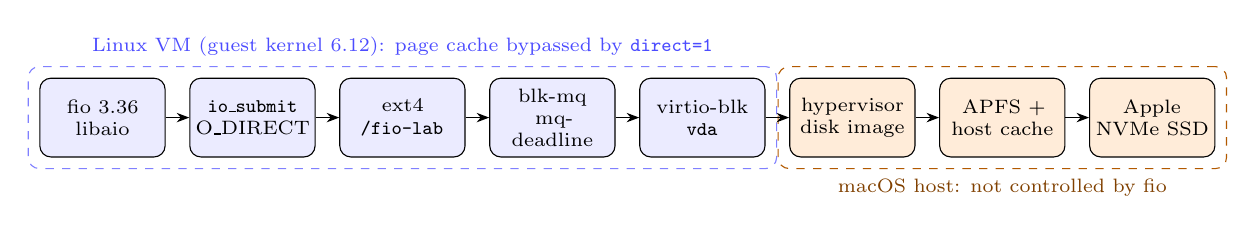
\begin{tikzpicture}[
  box/.style={draw,rounded corners,align=center,font=\scriptsize,minimum height=10mm,text width=14.5mm,inner sep=2pt},
  g/.style={box,fill=blue!8}, h/.style={box,fill=orange!15}, >={Stealth[length=1.6mm]}, node distance=3mm]
  \node[g] (fio) {fio 3.36\\libaio};
  \node[g,right=of fio] (sys) {\texttt{io\_submit}\\O\_DIRECT};
  \node[g,right=of sys] (fs) {ext4\\\texttt{/fio-lab}};
  \node[g,right=of fs] (blk) {blk-mq\\mq-deadline};
  \node[g,right=of blk] (vd) {virtio-blk\\\texttt{vda}};
  \node[h,right=of vd] (hv) {hypervisor\\disk image};
  \node[h,right=of hv] (apfs) {APFS +\\host cache};
  \node[h,right=of apfs] (ssd) {Apple\\NVMe SSD};
  \foreach \a/\b in {fio/sys,sys/fs,fs/blk,blk/vd,vd/hv,hv/apfs,apfs/ssd} \draw[->] (\a) -- (\b);
  \begin{scope}[on background layer]
    \node[draw=blue!50,dashed,rounded corners,fit=(fio)(vd),inner sep=4pt,
      label={[font=\scriptsize,blue!70]above:Linux VM (guest kernel 6.12): page cache bypassed by \texttt{direct=1}}] {};
    \node[draw=orange!70!black,dashed,rounded corners,fit=(hv)(ssd),inner sep=4pt,
      label={[font=\scriptsize,orange!50!black]below:macOS host: not controlled by fio}] {};
  \end{scope}
\end{tikzpicture}}
\caption{Path of one FIO request. \texttt{direct=1} removes the guest page cache only. The macOS side
can still cache or reorder I/O to the VM's disk image (tested in Section~\ref{sec:supp}).}
\label{fig:path}
\end{figure}

\subsection{Controls}

\begin{itemize}
  \item \textbf{Fixed for every main run:} \texttt{ioengine=libaio}, \texttt{direct=1}, \texttt{numjobs=1},
    \texttt{size=1g} (the same pre-written file), \texttt{ramp\_time=5s}, \texttt{runtime=30s},
    \texttt{time\_based=1}, \texttt{percentile\_list=50:95:99:99.9}. Within a case only \texttt{iodepth} changes.
  \item \textbf{Repetitions:} 3 per cell, 36 runs in total. The repetition loop is the \emph{outer}
    loop (A1 B1 C1 D1, then A2 \ldots). Slow drift such as SSD heat or background activity therefore spreads over all
    cases instead of biasing one.
  \item \textbf{Warm-up and cache:} the 1 GiB file was written once with real data before the first run, so
    reads hit allocated blocks (reading a sparse file returns zeros without any device I/O). \texttt{ramp\_time} drops the first 5\,s of each run.
  \item \textbf{Quiet machine:} all other containers in the Docker VM were stopped before the measured
    run. An earlier start with 18 project containers running was thrown away.
  \item \textbf{Validation:} every job file passes \texttt{fio -{}-parse-only} before the first run. All results are
    saved as JSON, and \texttt{analyze.py} builds the tables and plots from that JSON with no manual copying.
\end{itemize}

\begin{lstlisting}[caption={\texttt{jobs/B\_randrw70\_4k.fio} (header comment omitted). \texttt{run\_in\_container.sh} sets \texttt{ENGINE=libaio}, \texttt{SIZE=1g}, \texttt{RUNTIME=30}, \texttt{RAMP=5}, \texttt{FIO\_FILE=/fio-lab/db-test.bin} and \texttt{QD} $\in\{1,8,32\}$. The other cases differ only in \texttt{rw}, \texttt{bs} and \texttt{rwmixread}.}]
[global]
ioengine=${ENGINE}
direct=1
size=${SIZE}
runtime=${RUNTIME}
time_based=1
ramp_time=${RAMP}
group_reporting=1
filename=${FIO_FILE}
numjobs=1
iodepth=${QD}
percentile_list=50:95:99:99.9

[caseB]
rw=randrw
bs=4k
rwmixread=70
\end{lstlisting}

% ---------------------------------------------------------------------------
\section{Results}

\subsection{Required matrix (1 GiB file, mean of 3 runs)}

Table~\ref{tab:main} lists all 12 required cells. For the mixed cases B and C, IOPS and bandwidth are
read + write combined and the average latency is weighted by operation count. Percentiles are
completion latency (\texttt{clat}), shown as read / write. ``Depth'' is the bucket of fio's
\texttt{iodepth\_level} histogram that held 100\% of the I/Os, so \textbf{the requested queue depth was
reached in every run}. CV is the coefficient of variation of IOPS over the 3 repetitions.

\begin{table}[H]
\centering\small
\caption{Required experiments: 1 GiB file, \texttt{libaio}, \texttt{direct=1}, 30\,s per run, mean of 3 runs. Latency in \textmu s.}
\label{tab:main}
\begin{tabular}{@{}ccrrrrccc@{}}
\toprule
Case & QD & IOPS & CV\,\% & BW (MiB/s) & Avg lat & P95 (r / w) & P99 (r / w) & Depth \\
\midrule
\csname @@input\endcsname tables/main.tex 
\bottomrule
\end{tabular}
\end{table}

Several of these numbers are physically impossible for a laptop SSD. Case D reaches 20\,GiB/s and
case A 319k IOPS. In its last repetition, case A at QD\,1 averaged 30\,\textmu s per 4 KiB read. The high CV values in B and C point to the same
cause, which Table~\ref{tab:reps} makes clear: \textbf{the first repetition is almost always the slowest,
and later repetitions get faster}. Case A at QD\,1 runs at 11k, then 23k, then 33k IOPS.

\begin{table}[H]
\centering\small
\caption{IOPS for each repetition (repetitions were interleaved across cases, so rep 2 starts about 7 minutes after rep 1).}
\label{tab:reps}
\begin{tabular}{@{}ccrrrrr@{}}
\toprule
Case & QD & Rep 1 & Rep 2 & Rep 3 & Rep 3 / Rep 1 & CV \\
\midrule
\csname @@input\endcsname tables/reps.tex 
\bottomrule
\end{tabular}
\end{table}

\textbf{Explanation: the macOS host cache.} \texttt{direct=1} bypasses only the \emph{guest} page cache
(Figure~\ref{fig:path}). The VM's disk is a file on the Mac, and macOS caches that file in its own memory.
A 1 GiB working set fits easily in the Mac's 16 GiB. As the runs touch more of the file, more of it is served
from host RAM. This is exactly the trap from the lecture: ``if a file is served from RAM cache, are we
measuring the SSD?'' Case D is stable from the start because it streams the whole file every few
hundred milliseconds, so it is fully cached almost immediately.

\subsection{Same matrix with an 8 GiB file (closer to the device)}
\label{sec:supp}

To separate cache effects from device behaviour, I ran all 12 cells once more on an \textbf{8 GiB}
file (larger than the VM's 7.7 GiB RAM and half of the host's 16 GiB), with all other settings unchanged. This is one run per cell, and the file was written just before it,
so part of it may still sit in the host cache. These numbers are therefore an upper bound on what the SSD
path delivers, but much closer to it than the 1 GiB numbers.

\begin{table}[H]
\centering\small
\caption{1 GiB (mean of 3) against 8 GiB (1 run). ``Ratio'' = 1 GiB IOPS / 8 GiB IOPS. P99 is the worse of read and write. Latency in \textmu s.}
\label{tab:big}
\setlength{\tabcolsep}{4.5pt}
\begin{tabular}{@{}ccrrrrrrrrr@{}}
\toprule
 & & \multicolumn{3}{c}{IOPS} & \multicolumn{2}{c}{BW (MiB/s)} & \multicolumn{2}{c}{Avg lat} & \multicolumn{2}{c}{P99} \\
\cmidrule(lr){3-5}\cmidrule(lr){6-7}\cmidrule(lr){8-9}\cmidrule(l){10-11}
Case & QD & 1 GiB & 8 GiB & Ratio & 1 GiB & 8 GiB & 1 GiB & 8 GiB & 1 GiB & 8 GiB \\
\midrule
\csname @@input\endcsname tables/big.tex 
\bottomrule
\end{tabular}
\end{table}

With 8 GiB the picture looks like a real SSD seen through a VM. Random 4 KiB reads saturate at
$\approx$49k IOPS, sequential reads at $\approx$1.2 GiB/s, random-write-heavy work at $\approx$70 MiB/s, and
P99 reaches milliseconds. The 1 GiB results are 3--19$\times$ higher. \textbf{For PostgreSQL this gap is
the value of keeping the working set in memory} (\texttt{shared\_buffers} plus the OS cache). It is also why a
benchmark has to state its working-set size next to its results.

\begin{figure}[H]
\centering
\begin{tikzpicture}
\begin{groupplot}[group style={group size=2 by 2, horizontal sep=17mm, vertical sep=21mm},
  width=0.47\linewidth, height=5.0cm, xmode=log, log basis x=2, xtick={1,8,32}, xticklabels={1,8,32},
  xlabel={queue depth}, ymode=log, grid=major, grid style={gray!20}, tick label style={font=\scriptsize},
  label style={font=\small}, title style={font=\small\bfseries}, legend style={font=\scriptsize}]
\nextgroupplot[title={IOPS}, ylabel={IOPS},
  legend to name=leg, legend columns=6, legend style={draw=none,/tikz/every even column/.append style={column sep=6pt}}]
  \addplot[cA,thick,mark=*] table[x=qd,y=iops]{data/A.dat}; \addlegendentry{A}
  \addplot[cB,thick,mark=square*] table[x=qd,y=iops]{data/B.dat}; \addlegendentry{B}
  \addplot[cC,thick,mark=triangle*] table[x=qd,y=iops]{data/C.dat}; \addlegendentry{C}
  \addplot[cD,thick,mark=diamond*] table[x=qd,y=iops]{data/D.dat}; \addlegendentry{D}
  \addlegendimage{black,thick} \addlegendentry{1 GiB (mean of 3)}
  \addlegendimage{black,thick,dashed} \addlegendentry{8 GiB}
  \addplot[cA,thick,dashed,mark=o] table[x=qd,y=iops]{data/A_8g.dat};
  \addplot[cB,thick,dashed,mark=square] table[x=qd,y=iops]{data/B_8g.dat};
  \addplot[cC,thick,dashed,mark=triangle] table[x=qd,y=iops]{data/C_8g.dat};
  \addplot[cD,thick,dashed,mark=diamond] table[x=qd,y=iops]{data/D_8g.dat};
\nextgroupplot[title={Bandwidth}, ylabel={MiB/s}]
  \addplot[cA,thick,mark=*] table[x=qd,y=bw]{data/A.dat};
  \addplot[cA,thick,dashed,mark=*,mark options={fill=white}] table[x=qd,y=bw]{data/A_8g.dat};
  \addplot[cB,thick,mark=square*] table[x=qd,y=bw]{data/B.dat};
  \addplot[cB,thick,dashed,mark=square*,mark options={fill=white}] table[x=qd,y=bw]{data/B_8g.dat};
  \addplot[cC,thick,mark=triangle*] table[x=qd,y=bw]{data/C.dat};
  \addplot[cC,thick,dashed,mark=triangle*,mark options={fill=white}] table[x=qd,y=bw]{data/C_8g.dat};
  \addplot[cD,thick,mark=diamond*] table[x=qd,y=bw]{data/D.dat};
  \addplot[cD,thick,dashed,mark=diamond*,mark options={fill=white}] table[x=qd,y=bw]{data/D_8g.dat};
\nextgroupplot[title={Average latency}, ylabel={\textmu s}]
  \addplot[cA,thick,mark=*] table[x=qd,y=lat]{data/A.dat};
  \addplot[cA,thick,dashed,mark=*,mark options={fill=white}] table[x=qd,y=lat]{data/A_8g.dat};
  \addplot[cB,thick,mark=square*] table[x=qd,y=lat]{data/B.dat};
  \addplot[cB,thick,dashed,mark=square*,mark options={fill=white}] table[x=qd,y=lat]{data/B_8g.dat};
  \addplot[cC,thick,mark=triangle*] table[x=qd,y=lat]{data/C.dat};
  \addplot[cC,thick,dashed,mark=triangle*,mark options={fill=white}] table[x=qd,y=lat]{data/C_8g.dat};
  \addplot[cD,thick,mark=diamond*] table[x=qd,y=lat]{data/D.dat};
  \addplot[cD,thick,dashed,mark=diamond*,mark options={fill=white}] table[x=qd,y=lat]{data/D_8g.dat};
\nextgroupplot[title={P99 latency (worse of read/write)}, ylabel={\textmu s}]
  \addplot[cA,thick,mark=*] table[x=qd,y=worstp99]{data/A.dat};
  \addplot[cA,thick,dashed,mark=*,mark options={fill=white}] table[x=qd,y=worstp99]{data/A_8g.dat};
  \addplot[cB,thick,mark=square*] table[x=qd,y=worstp99]{data/B.dat};
  \addplot[cB,thick,dashed,mark=square*,mark options={fill=white}] table[x=qd,y=worstp99]{data/B_8g.dat};
  \addplot[cC,thick,mark=triangle*] table[x=qd,y=worstp99]{data/C.dat};
  \addplot[cC,thick,dashed,mark=triangle*,mark options={fill=white}] table[x=qd,y=worstp99]{data/C_8g.dat};
  \addplot[cD,thick,mark=diamond*] table[x=qd,y=worstp99]{data/D.dat};
  \addplot[cD,thick,dashed,mark=diamond*,mark options={fill=white}] table[x=qd,y=worstp99]{data/D_8g.dat};
\end{groupplot}
\end{tikzpicture}

\pgfplotslegendfromname{leg}
\caption{All four metrics against queue depth (log scales). Solid lines: 1 GiB file (mostly served from host cache).
Dashed lines: 8 GiB file (mostly reaches the SSD).}
\label{fig:main}
\end{figure}

\subsection{Mixed workloads by direction}

\begin{table}[H]
\centering\small
\caption{Cases B and C split into reads and writes (1 GiB, mean of 3). Latency in \textmu s.}
\label{tab:mixed}
\begin{tabular}{@{}ccrrrrrrrr@{}}
\toprule
 & & \multicolumn{2}{c}{IOPS} & \multicolumn{2}{c}{Avg lat} & \multicolumn{2}{c}{P99} & \multicolumn{2}{c}{P99.9} \\
\cmidrule(lr){3-4}\cmidrule(lr){5-6}\cmidrule(lr){7-8}\cmidrule(l){9-10}
Case & QD & read & write & read & write & read & write & read & write \\
\midrule
\csname @@input\endcsname tables/mixed.tex 
\bottomrule
\end{tabular}
\end{table}

\subsection{Finer queue-depth sweep (1 GiB, one 20\,s run per point)}

\begin{figure}[H]
\centering
\begin{tikzpicture}
\begin{groupplot}[group style={group size=2 by 1, horizontal sep=18mm},
  width=0.46\linewidth, height=4.8cm, xmode=log, log basis x=2, xtick={1,2,4,8,16,32,64,128},
  xticklabels={1,2,4,8,16,32,64,128}, xlabel={queue depth}, grid=major, grid style={gray!20},
  tick label style={font=\scriptsize}, label style={font=\small}, title style={font=\small\bfseries},
  legend style={font=\scriptsize, at={(0.03,0.97)}, anchor=north west}]
\nextgroupplot[title={Throughput relative to QD\,1}, ylabel={$\times$ QD\,1}, ymin=0]
  \addplot[cA,thick,mark=*] table[x=qd,y expr=\thisrow{iops}/29260.5]{data/sweep_A.dat}; \addlegendentry{A (IOPS)}
  \addplot[cD,thick,mark=diamond*] table[x=qd,y expr=\thisrow{bw}/3658.59]{data/sweep_D.dat}; \addlegendentry{D (MiB/s)}
\nextgroupplot[title={Average latency}, ylabel={\textmu s}, ymode=log]
  \addplot[cA,thick,mark=*] table[x=qd,y=lat]{data/sweep_A.dat}; \addlegendentry{A}
  \addplot[cD,thick,mark=diamond*] table[x=qd,y=lat]{data/sweep_D.dat}; \addlegendentry{D}
\end{groupplot}
\end{tikzpicture}
\caption{QD 1--128 on the 1 GiB file (one 20\,s run per point). A peaks at $\approx$11$\times$ QD\,1 (330k IOPS) at
QD\,32 and stays there, while its latency keeps doubling with every doubling of depth. D is noisier (the QD\,8
point is lower than QD\,4), which shows why single runs are not enough and the main matrix uses 3 repetitions.}
\label{fig:sweep}
\end{figure}

\subsection{Extension: WAL commit path (case E)}

\begin{table}[H]
\centering\small
\caption{Case E: 8 KiB sequential buffered writes, \texttt{fdatasync} after each one, 1 job, mean of 3 runs of 20\,s. Latency in \textmu s.}
\label{tab:wal}
\begin{tabular}{@{}crrrrrrr@{}}
\toprule
Case & Commits/s & MiB/s & Write avg & Write P99 & fdatasync avg & fdatasync P99 & \textmu s per commit \\
\midrule
\csname @@input\endcsname tables/wal.tex 
\bottomrule
\end{tabular}
\end{table}

The \texttt{write()} into the page cache takes 15\,\textmu s. The \texttt{fdatasync} that makes it durable
takes about 1\,ms on average and 5.5\,ms at P99. One PostgreSQL session committing one-row
transactions would therefore be capped at $\approx$1{,}000 commits/s by storage alone, no matter how fast the CPU is.

% ---------------------------------------------------------------------------
\section{Analysis}

\paragraph{1. Random read vs sequential read.}
At QD\,1 on the 8 GiB file, random 4 KiB reads (A) give 6.2k IOPS but only 24\,MiB/s.
Sequential 256 KiB reads (D) give fewer operations (3.9k IOPS) but 967\,MiB/s, which is 40$\times$ more data.
At QD\,32 the gap is 189 against 1{,}242\,MiB/s. Random access pays the full per-request cost (system call,
virtio, flash lookup) for only 4 KiB. Sequential access spreads that cost over 256 KiB and benefits from readahead
and large flash transfers. So random workloads should be judged by IOPS and latency, and scans by bandwidth.
For PostgreSQL: one 8 KiB page costs about 160\,\textmu s by random read but about 8\,\textmu s inside a
sequential scan ($258\,\mu s / 32$ pages), a ratio of about 20. PostgreSQL's default
\texttt{random\_page\_cost = 4} is far below this ratio because it assumes most random reads are cache hits.
That holds only while the working set fits in memory.

\paragraph{2. IOPS and latency as queue depth increases.}
Up to the point where the device saturates, more outstanding requests give more IOPS at almost
constant latency (8 GiB, case A: QD\,1$\to$8 gives 6.2k$\to$49.0k IOPS while latency stays 161$\to$163\,\textmu s).
After saturation, extra depth only adds queueing. QD\,8$\to$32 leaves IOPS at 48.5k but raises latency
4$\times$ to 659\,\textmu s. The measurements follow Little's law,
$\mathrm{IOPS} \approx \mathrm{QD} / \mathrm{latency}$: $32 / 659\,\mu s = 48.6$k and $8/163\,\mu s = 49.1$k, both
matching the measured values.

\paragraph{3. Does a higher queue depth always help? Where does scaling flatten?}
No. On the 8 GiB file \textbf{the random cases stop scaling at QD\,8}: A 49.0k$\to$48.5k, C 9.2k$\to$9.0k,
and B \emph{drops} from 19.0k to 17.4k. Sequential D gains only 14\% (1.06$\to$1.21\,GiB/s) for 4$\times$ the depth. Meanwhile P99 rises 2--4$\times$ in every case.
In the cached 1 GiB case the limit is CPU and memory copies rather than flash, so the plateau comes later:
Figure~\ref{fig:sweep} shows A flattening at QD\,32 ($\approx$330k IOPS, unchanged at 64 and only +6\% at 128,
where average latency is 365\,\textmu s). For PostgreSQL, more concurrent sessions than the storage can serve
add latency without adding throughput. This is one storage-side reason to cap active connections with a pooler
and to set \texttt{effective\_io\_concurrency} near the knee (around 8 here) rather than at its maximum.

\paragraph{4. Effect of the read/write ratio.}
More writes means less throughput and longer tails. On the 8 GiB file at QD\,8: 100\% read (A) gives 49.0k IOPS,
70\% read (B) gives 19.0k, and 30\% read with 8 KiB blocks (C) gives 9.2k. In bytes, B and C both land near
\textbf{70\,MiB/s} in total despite different mixes and block sizes, so the write share sets the pace. Writes cost more
because flash must program new pages and later erase blocks. In this setup each guest write also lands in a
growing, copy-on-write disk-image file on APFS. Reads in a mixed workload slow down too: their P99 in B and C
tracks the write P99 closely (Table~\ref{tab:mixed}), because reads queue behind writes. This is the storage-level
reason PostgreSQL spreads checkpoint writes over time (\texttt{checkpoint\_completion\_target}) instead of
writing everything at once.

\paragraph{5. Which workload has the highest P99, and why?}
On the 8 GiB file, \textbf{C at QD\,32 has the worst P99 (12.5\,ms for writes)}, followed by D at QD\,32
(10.6\,ms) and B at QD\,32 (8.6\,ms). In C, 70\% of the I/O are writes, and occasional
host flushes and garbage-collection pauses stall the whole queue. D's tail is mostly queueing arithmetic:
32 requests $\times$ 256 KiB = 8 MiB in flight at 1{,}242\,MiB/s is $\approx$6.4\,ms average wait (measured: 6.44\,ms), and P99 is the
unlucky end of that. In the 1 GiB runs the worst P99 is B at QD\,32 (2.2\,ms). That mean is dominated by
repetition 1, which ran before the host cache was warm (6.2\,ms against 0.2\,ms in reps 2--3), so a one-off
flush burst can dominate a tail metric. Throughout, the averages hide this: C at QD\,32 averages
3.6\,ms but its P99 is 3.5$\times$ higher.

\paragraph{6. Limitations of running FIO in a virtualised environment (Docker Desktop VM; WSL is similar).}
\begin{itemize}
  \item \textbf{Host cache.} \texttt{direct=1} only bypasses the guest cache. The 1 GiB results are 3--19$\times$
    the 8 GiB ones and drift between repetitions. On a bare-metal Linux server with O\_DIRECT this effect would not exist.
  \item \textbf{Misreported hardware.} The guest's \texttt{vda} reports \texttt{rotational=1} (a ``spinning disk'')
    although the real device is NVMe flash. Any software that tunes itself from this flag decides wrongly.
  \item \textbf{Extra layers.} virtio, the hypervisor, a sparse disk-image file and APFS each add latency and
    their own queues. The guest cannot see device SMART data, flash garbage collection or the real queue depth at the SSD.
  \item \textbf{Durability is not verifiable.} The guest's \texttt{fdatasync} becomes a flush of the
    disk-image file on macOS. Whether that reaches stable media (macOS needs \texttt{F\_FULLFSYNC} for that) cannot
    be checked from inside the VM, so case E is an optimistic number for commit latency.
  \item \textbf{Sandboxing.} Docker's default seccomp profile blocks \texttt{io\_uring\_setup}: fio failed with
    \texttt{err=1, io\_queue\_init: Operation not permitted}, so the io\_uring cross-check could not run without
    weakening container security. I documented the failure and did not disable seccomp.
  \item \textbf{Shared CPU.} The 10 vCPUs are shared with macOS. The run used 15--55\% of one vCPU, so CPU was not the
    limit, but other host activity can still add noise.
\end{itemize}

\paragraph{7. Why this is only an approximation of PostgreSQL.}
FIO models block traffic, not a database:
\begin{itemize}
  \item it runs no SQL, no query planner, no locks, no MVCC visibility checks and no buffer pool;
  \item real access is skewed (hot index roots stay cached) where FIO's offsets are uniform;
  \item PostgreSQL reads 8 KiB pages through the \emph{buffered} path, while cases A, B and D use 4 KiB or 256 KiB with \texttt{direct=1};
  \item the checkpointer writes in bursts, while FIO mixes reads and writes evenly;
  \item WAL group commit, full-page writes and autovacuum are missing.
\end{itemize}
The cases therefore give \emph{bounds}: how many page misses per second and how much scan bandwidth the
storage path can deliver, and how latency grows as concurrency rises. Turning that into transactions per second
needs a database benchmark such as \texttt{pgbench} on the same storage.

% ---------------------------------------------------------------------------
\section{Conclusions for the PostgreSQL deployment}

\begin{enumerate}
  \item \textbf{Size memory to the working set.} Keeping the hot data cached was worth 3--19$\times$ in IOPS
    and up to 16$\times$ in P99 here, more than any queue-depth or engine setting.
  \item \textbf{About 8 concurrent page misses saturate this storage.} Beyond that, extra sessions only add latency. Use a
    connection pooler and set \texttt{effective\_io\_concurrency} $\approx$ 8.
  \item \textbf{Write-heavy phases are the risk to tail latency} (C: 12.5\,ms P99). Spread checkpoints
    and run batch updates off-peak.
  \item \textbf{Commit latency is bound by \texttt{fdatasync}} ($\approx$1\,ms, P99 5.5\,ms). A WAL on a low-latency
    device, group commit, or \texttt{synchronous\_commit=off} for non-critical writes are the levers.
  \item \textbf{Measure on the real host.} The virtualised numbers show trends correctly but not absolute
    capacity. Rerun the same job files on the production-class Linux server before sizing hardware.
\end{enumerate}

% ---------------------------------------------------------------------------
\section{Reproducibility}

Everything is in \texttt{Lab-Task/10.FiOTools} (see \texttt{README.txt}): the five job files, the Dockerfile,
the runner scripts, all 36 main JSON outputs plus 33 supplementary ones, the run logs, \texttt{environment.txt}
and the CSV summaries.

\begin{lstlisting}[columns=fixed]
./scripts/run_all.sh all          # build image, run main + sweeps + 8 GiB + WAL (~45 min)
python3 -I scripts/analyze.py .   # JSON -> results/*.csv, report/tables, report/data
cd report && tectonic report.tex  # this PDF
\end{lstlisting}

Recorded environment: fio-3.36; Ubuntu 24.04.5 LTS container; kernel 6.12.54-linuxkit (aarch64); 10 vCPU;
7.7 GiB RAM in the VM; ext4 on \texttt{/dev/vda1} (mounted \texttt{rw,relatime,discard}); scheduler \texttt{mq-deadline};
\texttt{nr\_requests=256}; \texttt{max\_sectors\_kb=1280}. Host: Apple M4, 16 GiB, macOS 26.6.2, Docker Desktop 29.1.3.
Runs took place on 13 Nov 2026 between 16:06 and 16:47 UTC, with no other containers running.


\end{document}
